\documentclass[
	openany,
	% -- opções da classe memoir --
	12pt,				% tamanho da fonte
   % openright,
	%twoside,
    oneside,
    % para impressão em verso e anverso. Oposto a oneside
	a4paper,			% tamanho do papel. 
	brazil				% o último idioma é o principal do documento
	]{abntex2}

% ---
% Pacotes básicos 
% ---

\usepackage{fontspec}
\setmainfont{Arial}

\usepackage[utf8]{inputenc}		% Codificacao do documento (conversão automática dos acentos)
\usepackage{indentfirst}		% Indenta o primeiro parágrafo de cada seção.
\usepackage{listings}
\usepackage{color}% Controle das cores
\usepackage{graphicx}			% Inclusão de gráficos
\usepackage{microtype} 			% para melhorias de justificação
\usepackage{multicol}			% multiplas colunas no texto
\usepackage{subcaption}
\usepackage{caption}
\usepackage{float}
\usepackage{amsmath}
\usepackage{amssymb}
\usepackage{amsthm}
\usepackage{lipsum}
\usepackage{blindtext}
\usepackage{varwidth}
\usepackage{fancyvrb}
\usepackage{tcolorbox}
\usepackage{numberedblock}

\newcommand*\justify{%
  \fontdimen2\font=0.4em% interword space
  \fontdimen3\font=0.2em% interword stretch
  \fontdimen4\font=0.1em% interword shrink
  \fontdimen7\font=0.1em% extra space
  \hyphenchar\font=`\-% allowing hyphenation
}

\definecolor{eclipseBlue}{RGB}{42,0.0,255}
\definecolor{eclipseGreen}{RGB}{63,127,95}
\definecolor{eclipsePurple}{RGB}{127,0,85}
\lstdefinelanguage{Robo}
{
    keywords=[1]{
    },
    keywordstyle=[1]\color{eclipsePurple},
    keywords=[2]{},
    keywordstyle=[2]\color{eclipseBlue},
    sensitive=false,
    morestring=[b]',
    morecomment=[l]{--}
}
\lstset{
  language={Robo},
  basicstyle=\small\ttfamily, % Global Code Style
  captionpos=b, % Position of the Caption (t for top, b for bottom)
  extendedchars=true, % Allows 256 instead of 128 ASCII characters
  tabsize=2, % number of spaces indented when discovering a tab 
  columns=fixed, % make all characters equal width
  keepspaces=true, % does not ignore spaces to fit width, convert tabs to spaces
  showstringspaces=false, % lets spaces in strings appear as real spaces
  breaklines=true, % wrap lines if they don't fit
  frame=trbl, % draw a frame at the top, right, left and bottom of the listing
  frameround=tttt, % make the frame round at all four corners
  framesep=4pt, % quarter circle size of the round corners
  numbers=left, % show line numbers at the left
}

% ---
% ---
% Formatação de código-fonte
% ---
\usepackage{listings}

% Altera o nome padrão do rótulo usado no comando \autoref{}
\renewcommand{\lstlistingname}{Código}

% Altera o rótulo a ser usando no elemento pré-textual "Lista de código"
\renewcommand{\lstlistlistingname}{Lista de Códigos}

% Configura a ``Lista de Códigos'' conforme as regras da ABNT (para abnTeX2)
\begingroup\makeatletter
\let\newcounter\@gobble\let\setcounter\@gobbletwo
  \globaldefs\@ne \let\c@loldepth\@ne
  \newlistof{listings}{lol}{\lstlistlistingname}
  \newlistentry{lstlisting}{lol}{0}
\endgroup

\renewcommand{\cftlstlistingaftersnum}{\hfill--\hfill}

\let\oldlstlistoflistings\lstlistoflistings
\renewcommand{\lstlistoflistings}{%
   \begingroup%
   \let\oldnumberline\numberline%
   \renewcommand{\numberline}{\lstlistingname\space\oldnumberline}%
   \oldlstlistoflistings%
   \endgroup}
 
% ---

% Pacotes de citações
% ---
\usepackage[brazilian]{backref}	 % Paginas com as citações na bibl
\usepackage[alf]{abntex2cite}	% Citações padrão ABNT

% --- 
% CONFIGURAÇÕES DE PACOTES
% --- 

% ---
% Configurações do pacote backref
% Usado sem a opção hyperpageref de backref
\renewcommand{\backrefpagesname}{Citado na(s) página(s):~}
% Texto padrão antes do número das páginas
\renewcommand{\backref}{}
% Define os textos da citação
\renewcommand*{\backrefalt}[4]{
	\ifcase #1 %
		Nenhuma citação no texto.%
	\or
		Citado na página #2.%
	\else
		Citado #1 vezes nas páginas #2.%
	\fi}%
% ---

% ---
% Informações de dados para CAPA e FOLHA DE ROSTO
% ---
\titulo{Uma Abordagem para Tradução de uma Linguagem de Programação de Robôs para um Modelo Formal}
\autor{Iverson Luís Pereira}
\local{Recife}
\data{2018}
\orientador{Professor Sidney de Carvalho Nogueira}


\instituicao{%
	Universidade Federal Rural de Pernambuco -- UFRPE
  	\par
  	Departamento de Computação
    \par
  	Curso de Bacharelado em Ciência da Computação
}

\tipotrabalho{Trabalho de Conclusão de Curso}
% O preambulo deve conter o tipo do trabalho, o objetivo, 
% o nome da instituição e a área de concentração 
\preambulo{Monografia apresentada ao Curso de Bacharelado em Ciência da Computação da Universidade Federal Rural de Pernambuco, como requisito parcial para obtenção do título de Bacharel em Ciência da Computação.}
% ---


% ---
% Configurações de aparência do PDF final

% alterando o aspecto da cor azul
\definecolor{blue}{RGB}{41,5,195}

% informações do PDF
\makeatletter
\hypersetup{
     	%pagebackref=true,
		pdftitle={\@title}, 
		pdfauthor={\@author},
    	pdfsubject={\imprimirpreambulo},
	    pdfcreator={LaTeX with abnTeX2},
		colorlinks=true,       		% false: boxed links; true: colored links
    	linkcolor=blue,          	% color of internal links
    	citecolor=blue,        		% color of links to bibliography
    	filecolor=magenta,      		% color of file links
		urlcolor=blue,
		bookmarksdepth=4
}
\makeatother
% --- 

% --- 
% Espaçamentos entre linhas e parágrafos 
% --- 

% O tamanho do parágrafo é dado por:
\setlength{\parindent}{1.3cm}

% Controle do espaçamento entre um parágrafo e outro:
\setlength{\parskip}{0.2cm}  % tente também \onelineskip

% ---
% compila o indice
% ---
\makeindex
% ---

% ----
% Início do documento
% ----
\begin{document}

% Seleciona o idioma do documento (conforme pacotes do babel)
%\selectlanguage{english}
\selectlanguage{brazil}

% Retira espaço extra obsoleto entre as frases.
\frenchspacing 

% ----------------------------------------------------------
% ELEMENTOS PRÉ-TEXTUAIS
% ----------------------------------------------------------
% \pretextual
%\begin{figure}[h]
%\centering % este comando é usado para centralizar a figura
%
\includegraphics[width=7cm]{figuras/logo_ufrpe_horizontal.png}\\
%\end{figure}

% \begin{figure}[ht]
% \centering
% \begin{minipage}[b]{0.45\textwidth}
% 
\includegraphics[height=3cm]{figuras/logo_ufrpe_horizontal.png}
% \end{minipage}
% \qquad
% \begin{minipage}[b]{0.45\textwidth}
% 
\includegraphics[height=2.5cm]{figuras/logo_bsi.pdf}
% \end{minipage}
% \end{figure}

%\begin{minipage}[t]{1\textwidth}
	\begin{figure}[ht]
	    \hspace{4.5cm}
		
\includegraphics[height=3cm]{figuras/logo_ufrpe_horizontal.png}
	\end{figure}    
%\end{minipage}

% ---
% Capa
% ---
\imprimircapa
% ---
% ---
% Folha de rosto
% (o * indica que haverá a ficha bibliográfica)
% ---
\imprimirfolhaderosto
% ---

% dedicatoria
\begin{dedicatoria}
   \vspace*{\fill}
   \centering
   \noindent
   \textit{Dedico este trabalho aos meus amados pais, Rosânia e Ivanildo, e ao meu grande irmão, Igor. Os meus maiores presentes.\\} \vspace*{\fill}
\end{dedicatoria}

% agradecimentos
\begin{agradecimentos}
Agradeço à minha mãe, Rosânia, por sempre me apoiar e me incentivar nas horas mais difíceis. Obrigado por sua dedicação à família. Você é o meu maior tesouro, a minha maior fortaleza. Te amo, minha rainha.

Agradeço ao meu pai, Ivanildo, que tanto lutou e possibilitou a nossa família uma vida melhor na cidade grande. Onde, pude ter a oportunidade de ir a escola e mais tarde à Universidade. Tenho muito orgulho de você, pai. Te amo!

Agradeço ao meu grande e único irmão, Igor, a quem tenho muito carinho, e sua esposa Naiany por sempre estarem ao meu lado.

Agradeço aos meus avós, tias e primos(as), que de alguma forma contribuíram em minha jornada e compreenderam minha ausência pelo tempo dedicado aos estudos.

Aos amigos da vida pela força e torcida para que tudo desse certo. Especialmente, Artur, Igor, Kamila, Mariana e Osmar. Vocês são os irmãos que a vida me presenteou.

Ao meu orientador, Sidney Nogueira, pela dedicação, pela paciência, por acreditar e motivar nosso trabalho, pelo apoio constante e pela atenção durante todo o período de construção deste trabalho. A quem tenho grande admiração e respeito. Meu muito obrigado!

Ao meu tutor, Mike, e ao grupo PET-Ciranda da Ciência, por me incentivar nas atividades ensino, pesquisa e extensão, atividades essenciais durante minha trajetória acadêmica.

Meus sinceros agradecimentos a Universidade Federal Rural de Pernambuco e a todos os professores do curso de Bacharelado em Ciência da Computação. Aos meus amigos e companheiros de curso, em especial, Ana Juriti, Bruno Marques, Carlos Magnum, Danielly Queiroz, Jeremias Leite e Ricardo Luna. Algumas das pessoas mais inteligentes e fascinantes que tive a oportunidade de conviver.

Agradeço ao Núcleo de Tecnologia da Informação - NTI/UFPE que me deu a oportunidade de aplicar na prática todo o conhecimento que adquiri durante a minha graduação, além de aprender com colegas de trabalho incríveis.

Finalmente, agradeço à Deus por ter me dado forças e me fazer querer continuar. Sou extremamente grato à Ele, por ter me proporcionado momentos gloriosos com pessoas essenciais à minha vida e conquistado grandes oportunidades.


\end{agradecimentos}



% epigrafe
\begin{epigrafe}
    \vspace*{\fill}
	\begin{flushright}
		\textit{``A persistência é o caminho do êxito.'' \\
		(Charles Chaplin)}
	\end{flushright}
\end{epigrafe}

% resumo e abstract
\setlength{\absparsep}{18pt} % ajusta o espaçamento dos parágrafos do resumo
\begin{resumo}
 
O interesse por ambientes de programação de robôs para fins educacionais têm crescido nos últimos anos. No entanto, esses ambientes não possuem mecanismos automatizados para verificação dos programas, o que impossibilita que alunos e professores tenham um \textit{feedback} rápido e automático sobre o funcionamento dos programas. 
%Técnicas da Engenharia de Software são utilizadas para realizar verificação automática de software.
Verificação de Modelos é uma técnica da engenharia de software onde sistemas são especificados em uma linguagem formal com a finalidade de verificar as propriedades , assim, através de um verificador de modelos, provando formalmente a ausência de problemas. 
%Diante disso, programas precisam ser modelados em uma linguagem formal para que seja possível verificar automaticamente através um verificador de modelos.
Neste trabalho, programas escritos na linguagem de programação para a simulação de robôs chamada ROBO são traduzidos automaticamente para uma notação formal chamada CSP (\textit{Communicating Sequential Processes}) por meio de uma abordagem de tradução automatizada, onde, posteriormente, propriedades são verificadas em um verificador de modelos chamado FDR (\textit{Failures-Divergences Refinement}). A tradução foi implementada através de uma plataforma chamada Spoofax, onde definimos a gramática da linguagem ROBO e especificamos regras de transformação de ROBO para CSP. Além disso, validamos a abordagem utilizando uma ferramenta para verificar o comportamento de um programa ROBO com variáveis e procedimentos. %Desse modo, este trabalho propõe uma abordagem para a tradução automática da linguagem ROBO para o modelo formal CSP possibilitando a alunos e professores uma forma de apoio durante a programação nesses ambientes por meio de \textit{feedback} automático.
%Desse modo, este trabalho tem por objetivo propor uma abordagem de tradução automática de uma linguagem de programação de robôs para um modelo formal.

 \textbf{Palavras-chave}: Engenharia de Software, Verificação de Software, Métodos Formais, Verificador de Modelos, CSP, Tradução Automática, Spoofax.
\end{resumo}


\begin{resumo}[Abstract]
 \begin{otherlanguage*}{english}
  
There is an increasing interest in virtual robot programming environments for educational purposes in recent years. These environments are an alternative to the use of real robots, which have a high acquisition value. Automatic verification of robot programs is a demand of students and teachers that expect to have fast and automatic feedback about the correctness of robot programs. However, no free software provides an automatic verification of virtual robot programs.  This work proposes an approach for the automatic verification of virtual robot programs authored in the educational language called ROBO. We propose a compiler that reads programs written in ROBO and translates its source code into a formal notation called CSP (Communicating Sequential Processes), which is the input to a model checking tool called FDR (Failures-Divergences Refinement). The compiler was implemented using the facilities of the Spoofax framework, which is used to define a parser for the ROBO language and a set of translation rules from ROBO to CSP.
This work removes a limitation of our previous verification approach that does not perform the verification of ROBO programs containing variables and procedures.
A significant contribution is the extension of the verification approach to allow the automatic analysis of ROBO programs with variables and procedures.
The extension consists of the modification of the compiler grammar by the inclusion of variables and procedures and the inclusion of translation rules that define the formal semantics for the elements added into the grammar.
Moreover, the work proposes a tool that makes transparent the translation process from ROBO to CSP and the automatic verification using FDR. We validate the approach using the proposed tool to verify the behavior of a ROBO program with variables and procedures.

   \vspace{\onelineskip}
 
   \noindent 
   \textbf{Keywords}:  Software Engineering, Software Verification, Formal Methods, Model Checking, CSP, Automatic Translation, Spoofax.
 \end{otherlanguage*}
\end{resumo}

% ---
% inserir lista de ilustrações
% ---
\pdfbookmark[0]{\listfigurename}{lof}
\listoffigures
\cleardoublepage
% ---

% ---
% inserir lista de tabelas
% ---
\pdfbookmark[0]{\listtablename}{lot}
\listoftables*
\cleardoublepage
% ---

% ---
% inserir lista de listings
% ---
\pdfbookmark[0]{\lstlistlistingname}{lol}
\begin{KeepFromToc}
\lstlistoflistings
\end{KeepFromToc}
\cleardoublepage
% ---

% ---
% inserir lista de abreviaturas e siglas
% ---
\begin{siglas}
  \item[AST] \textit{Abstract Syntax Tree}
  \item[ATerm] \textit{Annotated Term Format}
  \item[CSP] \textit{Communicating Sequential Processes}
  \item[CTL] \textit{Computation Tree Logic}
  \item[DSL] \textit{Domain-Specific Language}
  \item[FDR] \textit{Failures-Divergences Refinement}
  \item[GUI] \textit{Graphical User Interface}
  \item[LTL] \textit{Linear Temporal Logic}
  \item[SGLR] \textit{Scannerless Generalized LR}
  \item[SVA] \textit{Shared Variable Programming}
  \item[TCTL] Lógica de Árvore de Cálculo Temporizado
\end{siglas}
% ---

% ---
% inserir o sumario
% ---
\pdfbookmark[0]{\contentsname}{toc}
\tableofcontents*
\cleardoublepage
% ---



% ----------------------------------------------------------
% ELEMENTOS TEXTUAIS
% ----------------------------------------------------------
\textual

% ----------------------------------------------------------
% inclusao das secoes do texto
% ----------------------------------------------------------
\chapter{Introdução}

O interesse da população pela robótica educacional vem aumentando nas últimas
décadas oferecendo benefícios em todos os níveis da educação, seja no ensino de crianças, adolescentes ou adultos (ALIMISIS, 2013). Um outro aspecto observado na literatura é que muitas aplicações de robótica são utilizadas para ajudar no aprendizado da matemática, ciência ou engenharia através de atividades práticas que envolvem a programação de robôs (BENITTI, 2012). A programação de robôs educacionais oferece apoio para o ensino e aprendizagem de programação, principalmente para aqueles que estão iniciando a construção do pensamento computacional, com o propósito de usar o raciocínio lógico para estruturar soluções coerentes para problemas complexos (BOMBASAR et. al, 2015).

Ambientes de programação de robôs são utilizados para a criação de atividades com
este fim, onde os ambientes são geralmente atrativos e lúdicos, assim pode despertar o fascínio e a curiosidade dos estudantes pela programação (SILVA et. al, 2014). Segundo o jornal Folha de Pernambuco (2016), o recente do uso desses ambientes de robótica na sala de aula como forma de apoio nas escolas públicas do estado de Pernambuco tem aumentado o interesse dos estudantes pelas disciplinas de matemática e física, ainda afirma que o uso efetivo da robótica educacional aumenta a criatividade, sociabilidade, a concentração e o senso de coletividade.

O ambiente de programação para o LEGO MindStorms é um exemplo de aplicação
com essa finalidade; apresenta uma interface para que o aluno possa escrever seus
programas e executar o programa em robôs educacionais. Um problema no uso da robótica educacional é o alto custo para adquirir equipamentos, como por exemplo, o robô MindStorms da LEGO. Uma alternativa para o uso de robôs é utilizar ambientes de robótica educacional baseados em simulação como o RoboMind. Estes ambientes permitem a simulação passo a passo do robô, a partir da execução dos comandos do programa,
ocasionando em uma melhor compreensão para o aluno (LESSA et al., 2015).

Um problema dos ambientes de simulação de robôs é que estes não oferecem um
mecanismo de verificação automática das soluções propostas por estudantes, ou seja, os programas escritos pelos alunos não são verificados quanto a sua corretude para o problema proposto, de modo que estudante e professor possam obter feedback automático sobre o funcionamento dos programas. O atual mecanismo de verificação em ambientes de simulação de robôs virtuais ocorre através da observação dos passos do robô, o que pode tornar uma tarefa demorada e trabalhosa. Além de onerosa, a verificação pode ser complexa. Por isso, métodos de verificação automática são tão importantes para determinar a corretude de um programa em diferentes perspectivas de maneira automatizada e rápida (DUARTE, 2011). 

Portanto, este trabalho propõe uma abordagem para a tradução automática de uma
linguagem de programação de robôs para um modelo formal com o objetivo de fornecer a
alunos e professores uma forma de apoio durante a programação nesses ambientes por meio de feedback automático. Além disso, este trabalho contribui para a área da Engenharia de Software através da junção da educação com a verificação de sistemas de software, por meio da abordagem proposta para resolver o problema descrito em seguida.

\chapter{Fundamentação Teórica}

\section{Métodos Formais}
\section{Verificador de Modelos}
\subsection{FDR}
\section{Linguagem de Domínio Específico}
\section{Processo de Compilação}
\subsection{Spoofax}
\chapter{Tradução de ROBO para CSP}
A Seção 3.1 descreve como foi realizado o processo de tradução automático de ROBO para CSP através do framework Spoofax. Desde a fase inicial da definição da gramática até a geração de código.

\section{Processo de Tradução Automática}

\subsection{Ferramentas e Ambiente de Programação}
O desenvolvimento de um compilador exige uma preparação bem elaborada de todo um ambiente de programação. No caso deste trabalho, foi necessário o uso do ambiente de programação Eclipse juntamente com um plugin do Spoofax. O qual foi essencial para o desenvolvimento da abordagem de tradução automática. O plugin tem todas as depedências para a geração de Árvore de Análise Sintática e transformação de código.

\section{Definição da Linguagem ROBO com Spoofax}
Nesta Seção veremos como ocorrreu todo o processo de definição da linguagem ROBO usando o framework Spoofax, o que inclui a definição da sintaxe e transformação da linguagem, resultando em código CSP.
\subsection{Definição da Sintaxe}
Essa é a etapa inicial para a construção do compilador, na qual devemos primeiro definir todos os aspectos sintáticos da linguagem de programação utilizada no ambiente RoboMind. Ou seja, essa etapa deverá ser capaz de considerar os programas escritos na linguagem ROBO e assegurá-los que estão sintaticamente corretos. Para a definição da gramática livre de contexto de ROBO foi utilizado o formalismo SDF3, como já explicado no Capítulo \ref{chap:cap2}. Além de definir a gramática, SDF3 também foi utilizado para definir a sintaxe lexical, como por exemplo, palavras reservadas de ROBO. O principal objetivo dessa etapa a geração de uma Árvore Sintática Abstrata (\textit{Abstract Syntax Tree - AST}, em inglês) dos programas ROBO. Esse produto resultante é de extrema importância para a geração de código CSP através do Stratego.

É importante saber que a linguagem ROBO possui algumas características que a difere das linguagens de programação comuns, uma vez que se trata de uma DSL, com um objetivo bem definido. Abaixo estão listadas algumas das principais características de ROBO:

\begin{itemize}
    \item Funções booleanas predefinidas para detecção de obstáculos ou objetos ao redor do robô, por exemplo \textit{frontIsObstacle}, para verificar se há obstáculo na frente do robô ou \textit{frontIsClear}, para verificar se a frente do robô está livre de quaisquer objetos.
    \item Funções predefinidas para a movimentação do robô, como por exemplo \textit{forward(n)}, para movimentar para frente ou \textit{backward(n)}, para movimentar para trás.
    \item Variáveis globais.
    \item Procedimentos parametrizados e não parametrizados.
    \item Estruturas condicionais e de repetição, assim como na maioria das linguagens de programação.
    \item Expressões aritméticas com valores inteiros.
\end{itemize}

Para exemplificar todo o processo de compilação, definimos um exemplo de programa em ROBO que resolve um problema específico. O problema definido foi o ``Contando Caixas'', proposto por RoboLab-FURB\ref{add-ref} e adaptamos para esta pesquisa. O objetivo desse problema é propor uma solução para a simulação de um robô capaz de contar caixas espalhadas por diferentes cenários. O problema foi alterado para que exista um parâmetro que determina o lado no qual o robô deverá contar, sendo lado esquerdo ou direito. Na Figura \ref{fig:map} é mostrado um mapa utilizado para a simulação do problema em questão. Nele é possível ver um robô e algumas caixas, duas na linha superior e três na linha inferior. Na figura foi adicionado um ``X'' para indicar a posição final que o robô deverá parar após a execução do programa. Para exemplificar uma simulação, considere que o lado direito foi escolhido como parâmetro, desse modo, o robô deverá percorrer em linha reta contando as caixas à sua direita e ao chegar na posição final mostrará o resultado 3, caso o parâmetro fosse o lado esquerdo, a quantidade de caixas contadas pelo robô seria 2.

\begin{figure}[h]
\centering
\caption{Exemplo de Mapa usado no RoboMind}
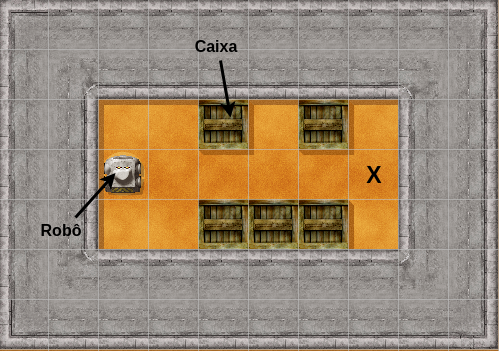
\includegraphics[height=7cm]{figuras/map2.png}
\fonte{O autor}
\label{fig:map}
\end{figure}

Na Figura \ref{fig:roboprogram} está disposto o código de um programa que resolve o problema da contagem de caixas. Esse programa possui duas variáveis globais: (a) \textit{countBoxes}, que é responsável por amazenar a quantidade de caixas; e (b) \textit{lookLine}, que é para indicar qual a linha que o robô deve contar as caixas (esquerda ou direita). Também há um procedimento parametrizado chamado \textit{countLine()}, este possui um único parâmetro denominado \textit{side}, o qual indicará o lado que o robô irá analisar. Se o valor passado ao parâmetro for igual a 1, então contará as caixas do lado esquerdo, se for qualquer valor diferente de 1, então contará as caixas do lado direito. O primeiro movimento do robô ocorre através do comando \textit{right} (indicado na linha 16), o qual altera sua orientação em 90 graus à direita. O próximo passo é a execução de um laço pelo comando \textit{repeatWhile}, a repetição ocorre enquanto não houver quaisquer objetos ou paredes na célula à frente do robô. Esse laço é responsável por chamar o procedimento \textit{countLine()} passando o valor da variável \textit{lookLine}, que neste exemplo tem valor 1, ou seja, contará as caixas da linha esquerda, seguindo de um \textit{forward} que move o robô para frente em uma unidade a cada execução do laço. Ao sair dessa estrutura de repetição, o procedimento será executado mais uma vez, com o objetivo de verificar possíveis caixas na última posição do robô e por fim a quantidade de caixas é exibida por meio do comando \textit{show} exibindo o valor armazenado na variável \textit{countBoxes} contendo a quantidade de caixas na linha de interesse. Este exemplo servirá para toda as etapas, desde a geração de uma AST, após a execução do parser, até a geração de código CSP, após a transformação da árvore.

\begin{figure}[h]
\caption{Programa escrito em ROBO}
\lstinputlisting{codes/program1.rob}
\fonte{O autor}
\label{fig:roboprogram}
\end{figure}

O trabalho \cite{nogueira}, como já mencionado, propõe um compilador que contempla a tradução de programas ROBO sem variáveis e procedimentos. No entanto, a gramática definida resulta uma AST é um formato  \texttt{Program(Sequence, Sequence)} similar a uma tupla, sendo assim, uma limitação, o que impossibilitava o uso de funções do framework Spoofax que facilitassem a transformação da árvore, como por exemplo, aplicação de filtros e recolhimento de termos específicos. Sabendo disso, para facilitar o trabalho em cima da árvore, foi necessário reconstruir partes da gramática de modo que a AST gerada tivesse um formato de lista, assim tornando possível o uso das funções nativas do Spoofax. Na Figura \ref{fig:gramatica_antes} tem um trecho da gramática definida no trabalho citado.

\begin{figure}[h]
\caption{Gramática escrita em forma de sequência}
\lstinputlisting[language=Java]{codes/gramatica_antes.sdf3}
\fonte{O autor}
\label{fig:gramatica_antes}
\end{figure}

Já na Figura \ref{fig:gramatica} a gramática foi totalmente reescrita, antes o que era \texttt{Sequence} tornou-se \texttt{Statement} seguido pelo operador * de concatenação. Dessa forma, ao invés do programa iniciar com uma \texttt{Sequence}, a qual também era seguido por uma \texttt{Sequence} precedida de uma \texttt{Instr}. Além dessa mudança, foi adicionado o termo \texttt{Declaration} (linha 6) que possui três tipos: \texttt{Variable}, \texttt{Procedure} e \texttt{ProcParam} (linhas 8, 9 e 12, respectivamente).

\begin{figure}[h]
\caption{Gramática escrita em forma de lista}
\lstinputlisting[language=Java]{codes/gramatica.sdf3}
\fonte{O autor}
\label{fig:gramatica}
\end{figure}

A definição da sintaxe é composta por módulos que podem ser importados e utilizados em outros módulos. Sabendo disso, o compilador de ROBO foi composto por 4 módulos: (1) \textit{Commom}, contendo toda a parte léxica da linguagem, como restrinções e palavras reservadas; (2) \textit{ExpressionsBoolean}, possuindo todas as definições da gramática para expressões booleanas; (3) \textit{ExpressionsMath}, contém a gramática livre de contexto e as prioridades de análise de cálculo matemático; e (4) \textit{Robo2CSP}, este é o módulo principal, pois engloba os demais, além de definir toda a gramática essencial da linguagem ROBO.

Um programa ROBO consiste em uma lista de declarações (\texttt{Statement}) que podem ser do tipo \texttt{Instr} ou \texttt{Declaration}. O tipo \texttt{Instr} contém todas as instruções básicas de ROBO, ou seja, é composta pelos comandos de movimentação, pintura de mapa, caputura de objetos e as estruturas condicionais e de repetição. Já o tipo \texttt{Declaration} é combinado de declarações para variáveis e para a declaração de procedimentos parametrizados e não parametrizados. Assim, está disposto na Figura \ref{fig:gramatica} parte do módulo Robo2CSP, nela estão definidas as produções da linguagem.

A produção \texttt{Statement.Declaration} define três alternativas para o tipo Declaration que estão definidas em três produções separadas, a primeira \texttt{Declaration.Varia\-ble}, para representar as variáveis, a segunda é \texttt{Declaration.Procedure}, para representar os procedimentos não parametrizados e por fim, \texttt{Declaration.ProcParam}, para representar elementos sintáticos de procedimentos parametrizados.

O corpo da produção para variáveis \texttt{<<Identifier> = <Expr>>} define uma declaração do tipo \texttt{Variable} composta de um identificador (\texttt{Identifier}), que é basicamente um texto descrevendo o nome da variável, seguido por um simbolo de igual e terminado por uma expressão que podem ser do tipo booleanas ou matemáticas (indicadas nas linhas 31 e 32 da Figura \ref{fig:gramatica}, respectivamente).

Para os procedimentos há duas produções, a primeira é para os procedimentos não parametrizados (\texttt{<proce\-dure <Identifier>\{ <Statement*> \}>}) que é composto pela palavra reservada \textit{procedure}, seguido por um identificador, que por sua vez é seguido por zero ou mais \texttt{Statement} entre um par de abre-fecha chaves. Já o segundo, para os procedimentos parametrizados, exige uma complexidade maior, uma vez que um procedimento pode ter \textit{n} parâmetros. A diferença do corpo (\texttt{<procedure <Identifier> <Params> \{ <Statement*> \}}) da produção desse tipo para o corpo do procedimento não parametrizado está na existência da produção \texttt{Params} (linha 28 da Figura \ref{fig:gramatica}) logo após o identificador. O corpo de \texttt{Params} é composto por zero ou mais identificadores separados por vírgula dentro dos símbolos de abre-fecha parênteses.

Uma vez definida as produções para declaração de procedimento, agora é necessário a definição de produções para chamada do mesmo. Esta produção está indicada na linha 34 da Figura \ref{fig:gramatica}. Uma chamada de procedimento nada mais é do que um subtipo de \texttt{Instr}, chamado de \texttt{ProcCall}. O corpo desta produção é composto por um identificador seguido pelos parâmetros, os quais são derivados de expressões. Por isso foi definido um novo tipo de produção, chamado de \texttt{ExprParams} que são \textit{n} expressões separadas por vírgula, entre um par de abre-fecha parênteses.

Descrito o passo a passo de como foi definida a gramática da linguagem ROBO. Agora, entra a etapa do \textit{parsing}, ou seja, o compilador consegue ler um programa escrito em ROBO e gerar sua Árvore Sintática Abstrata com todos os elementos do programa de modo estruturado. Consederando o programa ROBO mostrado na Figura \ref{fig:roboprogram}, geramos a sua AST após a execução do \textit{parsing}. A árvore está denotada pelas Figuras \ref{fig:ast1} e \ref{fig:ast2}, a primeira representa o programa, e a segunda representa o contéudo representado por reticências da linha 4 da figura anterior.

\begin{figure}[h]
\centering
\caption{Geração da AST do programa ROBO}
\lstinputlisting[language=Java]{codes/ast2.aterm}
\fonte{O autor}
\label{fig:ast1}
\end{figure}

\begin{figure}[h]
\centering
\caption{Geração de uma AST do procedimento \textit{countLine()}}
\lstinputlisting[language=Java]{codes/ast1.aterm}
\fonte{O autor}
\label{fig:ast2}
\end{figure}

A geração da AST é essencial para a etapa de geração de código através do Stratego. O Stratego precisa de uma uma árvore como entrada em um formato que facilite sua análise, por isso que as ASTs são representadas em um formato textual, como visto anteriormente. Esse formato é denominado de Formato de Termo Anotado (\textit{Annotated Term Format - ATerm, em inglês}) e cada elemento da árvore é chamado de \textit{Term}. Sabendo disso, a próxima Seção descreve o passo a passo de como é realizada a análise da árvore e como foram definidas as regras de compilação para a geração de código CSP em cima dos \textit{ATerms}.

\subsection{Transformação com Stratego}

Essa etapa é a mais importante, em razão de que o resultado deste processo é o código CSP, produto essencial para a verificação dos programas ROBO semanticamente equivalentes à ROBO no verificador de modelos FDR.

O primeiro passo foi definir uma regra em Stratego para manipular os principais termos de um AST. No qual, para cada termo, outras regras são aplicadas, isto é, o conjunto resultante de termos aplicados à uma regra é utilizado pela regra consecutiva. Isto é melhor exemplificado na regra definida na Figura \ref{fig:rules}. A regra \texttt{to-csp} é reponsável por aplicar um cabeçalho para os programas em CSP e desencadear outras regras para os demais termos da árvore. Como a AST de ROBO sempre inicia com \texttt{Program}, isso siginifica que toda geração de código é iniciada por essa regra, no caso ocorre o casamento com o termo \texttt{Program(T1)}, indicado na linha 4, onde \texttt{T1} é todo o restante da árvore sintática. Diante disso, todas as demais regras são aplicadas aos termos derivados de \texttt{T1}.

\begin{figure}[h]
\centering
\caption{Regra inicial para um programa ROBO}
\lstinputlisting{codes/rules.str}
\fonte{O autor}
\label{fig:rules}
\end{figure}

Antes de arbordar sobre as demais partes da regra, vale salientar que o modelo formal de ROBO, especificados em CSP, proposto por \cite{nogueira} possui um processo que simula uma memória devido à impossibilidade de utilizar variáveis em CSP. Por isso, esse processo é utilizado para armazenar apenas os valores da posição (x,y) do robô, sua orientação e a posição (x,y) de um determinado objeto no mapa que são consultados e atualizados em tempo de execução. Diante disso, este trabalho vai reutilizar esta mesma memória para armazenar os valores das variáveis encontradas em programas ROBO, bem como os valores dos parâmetros dos procedimentos. No entanto, na espeficicação formal do trabalho citado anteriormente, os valores dos atributos do robô, citados neste parágrafo, são representados por um conjunto de dados, no formato de chave e valor, para inicialização da memória: \texttt{INIT = \{ (X, startX), (Y, startY), (ORIENTATION, NORTH\_), (BX, startBX), (BY, startBY) \}}. Assim, propomos neste trabalho uma abordagem para que todas as variáveis presentes em programas ROBO sejam adicionadas à esse conjunto \texttt{INIT}. Por exemplo, as variáveis \texttt{countBoxes} e \texttt{lookLine} do programa ilustrado na Figura \ref{fig:roboprogram} seriam adicionadas ao conjunto da seguinte forma: \texttt{INIT = \{ (countBoxes, 0), (lookLine, 1), (X, startX), (Y, startY), (ORIENTATION, NORTH\_), (BX, startBX), (BY, startBY) \}}. 

Sabendo disso, como visto na Figura \ref{fig:rules}, está definida a regra \texttt{to-csp} na qual o conteúdo que está entre as linhas 5 e 13 será transformado em código CSP. A linha 5 contém o elemento \texttt{vars'} que é utilizado para transformar todas as variáveis de ROBO em constantes no código CSP. Esse elemento é transformado após a palavra \texttt{with}, no qual outras duas regras são aplicadas em \texttt{T1} e o valor resultante é aplicado a \texttt{vars'}. Inicialmente é aplicado a regra \texttt{<get-vars>} em \texttt{T1}, essa regra tem como objetivo filtrar o conjunto de \textit{ATerms} que casam com o termo \texttt{Declaration(Variable(\_,\_))}, olhar linha 6 da Figura \ref{fig:rules2}. Após isso, uma lista com todos os termos desejados são aplicados na regra mais a esquerda, \texttt{<var-analyze-global>}, que é encarregada de escrever as variáveis declaradas no programa ROBO em forma de constantes na especificação formal CSP. A Figura \ref{fig:rules_constants} mostra a definição das regras responsáveis pela geração das constantes. A regra \texttt{<var-analyze-const>} é aplicada de modo recursivo, muito similar às funções de linguagens funcionais, no qual uma função é aplicada na cabeça (\textit{head}) enquanto a mesma função é aplicada na calda (\textit{tail}) até chegar no caso base, que neste é caso é uma lista vazia, como está indicado na linha 3. A análise ocorre em cima do termo \textit{Declaration(var)}, onde a regra \texttt{<write-variable-const>} é aplicada em \texttt{var} para escrever o CSP correspondente ao tipo de dado da variável. Por isso, há três declarações dessa regra, a primeira para escrever um texto vazio em casos de expressões matemáticas, já que as constantes não recebem expressões (exemplo, a + b); a segunda para escrever o texto \texttt{[name]Const = [v]}, ou seja, o nome da variável (\texttt{name}) e seu respectivo valor inteiro (\texttt{v}); por último, para expressões booleanas, onde uma outra regra, \texttt{<to-csp-e>}, é aplicada para escrever o valor booleano (\textit{true} ou \textit{false}), dependendo do valor do termo em \texttt{exp'}.

\begin{figure}[h]
\centering
\caption{Regras para geração de constantes em CSP}
\lstinputlisting{codes/rules_constants.str}
\fonte{O autor}
\label{fig:rules_constants}
\end{figure}

Outro ponto a destacar está na linha 6 da Figura \ref{fig:rules}, no qual \texttt{MAXVAR} indica os limites inferior e superior que as variáveis poderão antigir durante a execução do programa em FDR, pois em CSP se o conjunto númerico for muito grande, a verificação poder ter o desempenho comprometido devido a grande quantidade de estados que o programa possui. Ainda em relação as variáveis, está declarado na linha 7, o tipo de dados \texttt{VarType}, que em CSP atribui os tipos dos parâmetros (\texttt{paramsType'}) e das variáveis (\texttt{varsType'}) encontrados nos programas ROBO.

\begin{figure}[h]
\centering
\caption{Conjunto de regras auxiliares}
\lstinputlisting[language=Java]{codes/rulesAux.str}
\fonte{O autor}
\label{fig:rules2}
\end{figure}

Para gerar código CSP em relação ao tipo de dados para parâmetros e variáveis através dos elementos \texttt{paramsType'} e \texttt{varsType'} é necessário aplicar algumas regras para recolher os termos de interesse na árvore sintática. A primeira regra aplicada ocorre em \texttt{paramsType'}, ver linha 8 da Figura \ref{fig:rules2}. A regra \texttt{<get-params>} aplica uma função nativa do \textit{Stratego}, chamada de \texttt{collect-all}, cujo objetivo é recolher todos os termos por meio de uma busca por toda árvore AST, o que inclue os nós e seus respectivos filhos. O retorno dessa função é uma lista contendo todos os termos \texttt{Params(\_)} do programa ROBO que, em seguida,  é aplicada à regra \texttt{<get-ids>} que de modo similar a regra anterior recolhe todos os termos contendo os identificadores (\texttt{ID(\_)}) dos parâmetros. Após todo esse processo de filtragem de termos, ocorre a escrita de texto, ou seja, o código CSP é gerado. Na Figura \ref{fig:rules_param_type} está destacada a implementação da regra \texttt{<param-analyze-type>} que é aplicada na lista gerada após a aplicação da regra \texttt{<get-ids>}, como foi bem colocado.

Essa regra é aplicada também de modo recursivo, a recursão ocorre na linha 4, onde o primeiro elemento da lista \texttt{ID(n)} é analisado e destinado a regra \texttt{<write-param\-type>} que é aplicada em \texttt{n}, enquanto para o restante da lista (\texttt{es}) a regra principal é aplicada recursivamente. A regra \texttt{write-param-type} escreve o código CSP, todo o contéudo que está entre os síbmbolos crifrão e colchetes é convertido em texto e \texttt{[n]} é substituído pelo nome do parâmetro analisado. Para exemplificar, o termo \texttt{ID("side")}, visto na linha 4 da Figura \ref{fig:ast2}, é escrito em CSP como \texttt{side.MAXVAR} após todo esse processo descrito, o mesmo vale para todos os parâmetros em qualquer código ROBO.

\begin{figure}[h]
\centering
\caption{Regras para os tipos de dados de parâmetros em código CSP}
\lstinputlisting[language=Java]{codes/rules_param_type.str}
\fonte{O autor}
\label{fig:rules_param_type}
\end{figure}

De modo semelhante ao que é feito em \texttt{paramsType'}, também ocorre em \texttt{vars\-Type'}. A diferença está em como ocorre a escrita de código CSP, uma vez que as variáveis ROBO possuem dois tipos de dados em suas expressões: \texttt{Bool}, para expressões com valores booleanos e \texttt{MAXVAR}, para expressões com valores inteiros. A regra \texttt{<write-variable-type>}, como mostra nas linhas 6 e 9 da Figura \ref{fig:rules_var_type}, aparece duas vezes, a primeira para termos que possuem expressões matemáticas e a segunda para os termos com expressões booleanas.

\begin{figure}[h]
\centering
\caption{Regras para os tipos de dados de variáveis em código CSP}
\lstinputlisting[language=Java]{codes/rules_var_type.str}
\fonte{O autor}
\label{fig:rules_var_type}
\end{figure}

Foi explicado alguns paráfragos antes, que em CSP é necessário um processo para simular uma mémória que armazena os valores das variáveis e demais dados do robô. Assim, a escrita do CSP de parâmetros e variáveis em \texttt{INIT}, através dos elementos \texttt{paramsInit'} e \texttt{varsInit'}, ocorre de modo análago às explicações dadas para os tipos de dados de parâmetros e variáveis.



....



\chapter{Implementação} %não sei como chamar este capitulo
\label{chap:cap4}
Este capítulo tem por objetivo mostrar como seria uma protótipo funcional que possibilite a integração do FDR com o compilador desenvolvido nesta pesquisa através dos serviços. Na Seção \ref{sub:exper} é explicado como foi realizado o experimento através de um protótipo que integra o compilador com o verificador de modelos. Na Seção \ref{sub:results} é apresentado os resultados obtidos usando a ferramenta proposta.

\section{Experimento Realizado}
\label{sub:exper}

No Capítulo \ref{chap:cap3} foi apresentado um exemplo (Contando Caixas) adaptado de \cite{furb} que foi utilizado para exemplificar durante o processo de definição sintática e transformação. Para este experimento, vamos utilizar esse mesmo exemplo, no entanto, em sua versão completa.

%Um dos objetivos desta pesquisa é o desenvolvimento de um protótipo funcional de uma ferramenta que integre o compilador com o verificador de modelos de modo transparente ao usuário do RoboMind.
Propomos um protótipo desenvolvido em Java que provê as principais funcionalidades para a verificação automática dos programas ROBO. Implementamos uma classe chamada \texttt{RobotChecker} com três métodos. O método \texttt{translateRobo2CSP} é responsável por realizar a tradução do programa ROBO para sua a representação formal em CSP; o método \texttt{translateMap2CSP} realiza a tradução do mapa para a notação CSP; e \texttt{verifyAssertion} que faz a verificação das propriedades por meio dos serviços de FDR.

Listamos as principais funcionalidades do protótipo implementado:

\begin{itemize}
    \item Tradução de ROBO para CSP: recebe um programa ROBO como entrada e através da API do Spoofax é realizada a tradução usando o compilador desenvolvido por esta pesquisa; e como saída é gerado a especificação do programa em notação CSP.
    \item Tradução de mapa: recebe um mapa do ambiente RoboMind como entrada e realiza a tradução automática; e como saída é gerado a especificação formal em CSP do mapa.
    \item Verificação das propriedades no FDR: recebe como entrada o mapa e o programa escritos em CSP, resultado da tradução automatizada; e como saída gera os resultados das verificações e os \textit{traces} resultantes, se houver.
\end{itemize}

%\section{Definição do problema}
\label{sec:defprob}
O problema consiste em um mundo de 6 colunas e 3 linhas, onde o robô sempre inicia na primeira coluna da segunda linha e e com caixas distribuídas aleatoriamente na primeira e última linha. O objetivo é fazer o robô andar até a última coluna e mostrar alguns valores inteiros através do comando \texttt{show}. O primeiro e segundo valor representam a quantidade de caixas na primeira e última linha, respectivamente. O terceiro valor mostrado mostra quais das duas linhas possuem mais caixas: sendo o valor 1 para a primeira linha, o valor 2 para a última e valor 3 se ambas possuem a mesma quantidade. O quarto valor exibido é a diferença de caixas entre as duas linhas. O quinto e último valor, respectivamente, representa a linha na qual apareceu a primeira e última caixa: sendo valor 1 para a primeira linha; valor 2 para a segunda; e valor 3 para ambas. Para ilustrar o experimento, considere os mapas apresentados na Figura \ref{fig:problem}, para cada um dos mapas tem-se a saída esperada no término da execução do programa.

\begin{figure}[h]
\centering
\caption{Mapas e saídas esperadas do problema ``Contando Caixas"}
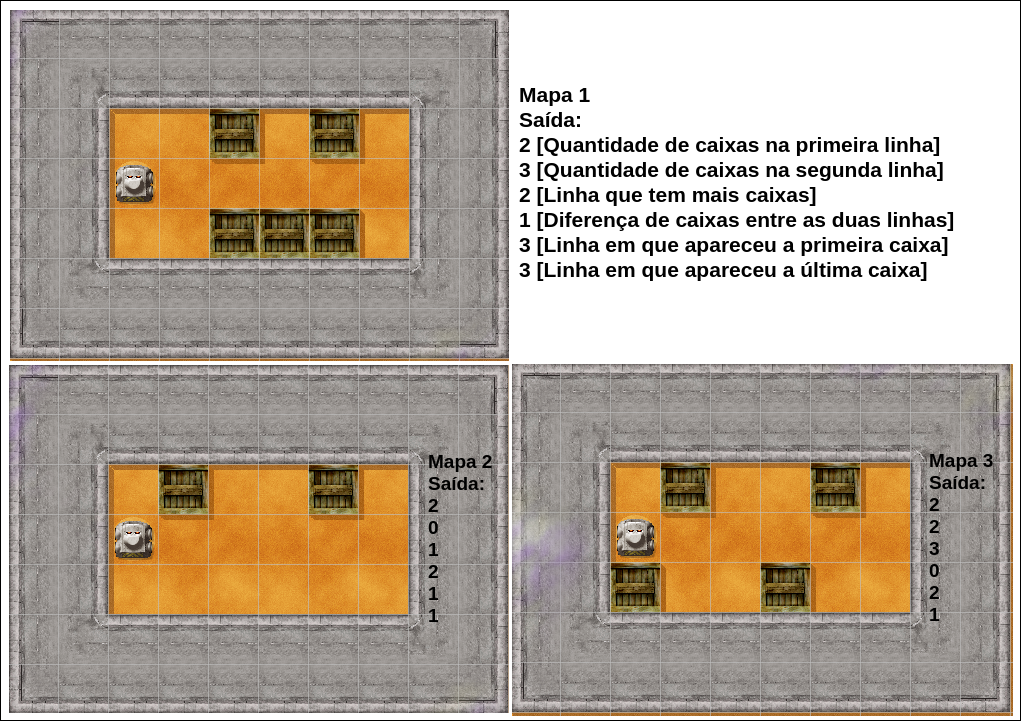
\includegraphics[height=10cm]{figuras/problema.png}
\fonte{\cite{furb}}
\label{fig:problem}
\end{figure}

Apresentado o problema, o próximo passo foi desenvolver uma solução para esse problema. Então desenvolvemos um programa ROBO capaz de apresentar as mesmas saídas para cada um desses mapas. A solução que propusemos contém cinco procedimentos e algumas variáveis que são suficientes para resolver o problema em questão. A Figura \ref{fig:solution} apresenta um trecho do código ROBO proposto. Podemos notar que há uma estrutura de repetição (\texttt{repeatWhile}) com uma condição (\texttt{frontIsClear}) que verifica se a célula posterior ao robô está livre. Os cinco procedimentos definidos são: (1) \texttt{countLeft}, conta a quantidade de caixas à esquerda do robô; (2) \texttt{countRight}, conta a quantidade de caixas à direita do robô; (3) \texttt{showsMoreBoxes}, mostra qual linha tem mais caixas e a diferença entre elas; (4) \texttt{getBoxsFirstLine}, mostra a quantidade de caixas na primeira linha; por fim, (5) \texttt{getBoxLastLine}, mostra a quantidade de caixas na última linha.

\begin{figure}[h]
\centering
\caption{Solução proposta em ROBO para o problema Contando Caixas}
\lstinputlisting{codes/solution.rob}
\fonte{O autor}
\label{fig:solution}
\end{figure}

Para validar a efetividade do compilador integrado ao FDR, foi necessário verificar as saídas geradas pelo protótipo e executar os \textit{traces} no ambiente RoboMind, obtidos através do resultado da verificação da propriedade: \texttt{assert PROGRAM :[deadlock free [F]]}. Na próxima seção estão descritos os resultados gerados pela ferramenta.

Definimos três testes, um para cada mapa. Na Tabela \ref{table:map1} estão dispostas as entradas e saídas geradas após a execução de cada método. Para o método \texttt{translateRobo2CSP} o arquivo \texttt{program.robo} (o mesmo da Figura \ref{fig:solution}) e  como saída obtivemos o arquivo \texttt{program.csp} com a especificação formal do programa ROBO.

\begin{table}
\caption{Entradas e saídas para o mapa 1}
\resizebox{\textwidth}{!}{%
\begin{tabular}{*{14}{|c}|}
\hline
\multicolumn{3}{|c|}{\textbf{Map 1}} \\ \hline
\textbf{method} & \textbf{input} & \textbf{output} \\ \hline
translateRobo2CSP & program.robo & program.csp \\ \hline
translateMap2CSP & map1.map & map1.csp \\ \hline
verifyAssertion & program.csp, map1.csp, test1\_program\_map1.csp & result1, traces1 \\ \hline
\end{tabular}%
}
\label{table:map1}
\fonte{O autor}
\end{table}

\begin{table}[]
\label{tab:map2}
\caption{Entradas e saídas para o mapa 2}
\resizebox{\textwidth}{!}{%
\begin{tabular}{*{14}{|c}|}
\hline
\multicolumn{3}{|c|}{\textbf{Map 2}} \\ \hline
\textbf{method} & \textbf{input} & \textbf{output} \\ \hline
translateRobo2CSP & program.robo & program.csp \\ \hline
translateMap2CSP & map2.map & map2.csp \\ \hline
verifyAssertion & program.csp, map2.csp, test2\_program\_map2.csp & result2, traces2 \\ \hline
\end{tabular}%
}
\fonte{O autor}
\end{table}

\begin{table}[]
\label{tab:map3}
\caption{Entradas e saídas para o mapa 3}
\resizebox{\textwidth}{!}{%
\begin{tabular}{*{14}{|c}|}
\hline
\multicolumn{3}{|c|}{\textbf{Map 3}} \\ \hline
\textbf{method} & \textbf{input} & \textbf{output} \\ \hline
translateRobo2CSP & program.robo & program.csp \\ \hline
translateMap2CSP & map3.map & map3.csp \\ \hline
verifyAssertion & program.csp, map3.csp, test3\_program\_map3.csp & result3, traces3 \\ \hline
\end{tabular}%
}
\fonte{O autor}
\end{table}

\section{Resultados}
\label{sub:results}
...
\begin{table}[]
\caption{Resultado obtido após a verificação do FDR}
\resizebox{\textwidth}{!}{%
\begin{tabular}{*{14}{|c}|}
\multicolumn{1}{c}{Map 1} & \multicolumn{1}{c}{Map 2} & \multicolumn{1}{c}{Map 3} \\
assert PROGRAM :{[}deadlock free {[}F{]}{]} & assert PROGRAM :{[}deadlock free {[}F{]}{]} & assert PROGRAM :{[}deadlock free {[}F{]}{]} \\
Result: Failed & Result: Failed & Result: Failed \\
Counterexample - Traces: & Counterexample - Traces: & Counterexample - Traces: \\
right() & right() & right() \\
forward(1) & forward(1) & forward(1) \\
forward(1) & forward(1) & forward(1) \\
forward(1) & forward(1) & forward(1) \\
forward(1) & forward(1) & forward(1) \\
forward(1) & forward(1) & forward(1) \\
show(2) & show(2) & show(2) \\
show(3) & show(0) & show(2) \\
show(2) & show(1) & show(3) \\
show(1) & show(2) & show(0) \\
show(3) & show(1) & show(2) \\
show(3) & show(1) & show(1)
\end{tabular}%
}
\fonte{O autor}
\end{table}

Levando-se em conta o que foi observado, para os três mapas analisados, comparando as saídas geradas pelo RoboMind e pela ferramenta proposta, é notório que a tradução do programa foi realizado corretamente, isto é, os programas CSP são representados semanticamente equivalentes a ROBO.



\chapter{Conclusão}
\label{chap:cap5}
%escrever minha conclusao

\section{Trabalhos Relacionados}

O único trabalho encontrado na literatura que realiza verificação de programas de robôs educacionais de forma totalmente automática é~\cite{nogueira}. Porém encontramos outro trabalho que usa verificação automática no contexto educacional. O artigo~\cite{SVA} propõe SVA (\textit{Shared Variable Programming}), que é uma ferramenta para o aprendizado de programação concorrente usando uma linguagem educacional; esta ferramenta integra um compilador da linguagem educacional para um modelo CSP com o verificador de modelos FDR. SVA permite analisar propriedades de programas concorrentes como, por exemplo, se os programas entram ao mesmo tempo em uma região crítica. Além disso, a ferramenta possui uma interface gráfica que apresenta os resultados das verificações retornados por FDR de uma forma amigável para o usuário. Esse trabalho mostra que é possível utilizar o FDR e CSP para a criação de ferramentas de verificação automática de linguagens de domínio específico. 

Em \cite{emanuel2017}, é proposto um protótipo de um ambiente para avaliação automática de robôs virtuais. Esse trabalho é uma continuação do trabalho \cite{nogueira} com foco no projeto e prototipação da interface gráfica de um ambiente para avaliação automática de robôs virtuais. O ambiente proposto objetiva a avaliação de forma automática e \textit{feedback} sobre o funcionamento dos programas escritos em ROBO, através de uma interface gráfica que lembra um sistema de julgamento online (\textit{Online Judgment System}) utilizados nas maratonas de programação. A implementação deste ambiente depende diretamente de um dos produtos deste trabalho, que é a extensão do compilador de ROBO para CSP e sua integração com a ferramenta FDR.

O trabalho \cite{silva} apresenta um método para a verificação automática durante a simulação de futebol de robôs, esse trabalho considera a especificação formal e a verificação de planos de um time de robôs simulados. A simulação ocorre de modo que vários robôs estão executando ao mesmo tempo e propondo uma solução conjunta, onde o autor denomina como sistemas multiagente. Nesse trabalho é utilizado um verificador de modelos para analisar algumas propriedades, dentre elas estão a verificação de ausência de \textit{deadlocks} e/ou \textit{livelocks} levando em consideração o tempo, pois o tempo é um fator essencial a ser considerado durante a verificação da simulação de futebol de robôs.  Por este motivo é utilizado o verificador de modelos chamado UPPAAL que oferece um conjunto de ferramentas para a verificação de sistemas em tempo real utilizando autômatos, além de utilizar uma linguagem chamada TCTL (Lógica de Árvore de Cálculo Temporizado) para formalizar as propriedades esperadas para o sistema. A diferença desse trabalho mostrado para esta proposta de pesquisa é que a verificação automática considera o tempo e sua abordagem foi desenvolvida especificamente para sistemas onde vários agentes atuam simultaneamente e por isso faz uso de uma outra ferramenta de verificação diferente da FDR.
	
\citeonline{SSS147734} propõe a verificação formal de robôs para assistência pessoal. Esses robôs estão presentes nas casas das pessoas e as ajudam em suas tarefas diárias, e como se trata de interação real com pessoas é necessária uma garantia de segurança, para que esses robôs não causem nenhum dano ou se coloquem em situações inesperadas. Por isso, é proposto um método de verificação formal. Essa proposta utiliza um verificador de modelos chamado SPIN que é bastante utilizado em sistemas de missões espaciais, telecomunicação e engenharias. A linguagem desse verificador é chamada PROMELA. Também foi utilizada uma linguagem chamada Brahms para modelar o robô. O processo de verificação ocorre quando o modelo escrito em Brahms é traduzido para linguagem PROMELA, onde o verificador de modelos pode verificar se as propriedades são satisfeitas ou não. Um exemplo de propriedade é saber se o robô irá se mover para cozinha quando o usuário envia o comando ao robô.  Essas propriedades são baseadas e pensadas na simulação e validação do usuário final, com o objetivo de aumentar a segurança prática e a confiabilidade dos assistentes robotizados, já que se trata de robôs físicos que estão trabalhando com pessoas reais. O processo de verificação é similar a esta proposta de pesquisa em alguns pontos, um deles é a tradução da linguagem modelada de um robô para uma especificação formal através de um compilador, contudo essa abordagem se trata de uma simulação voltada para o mundo real, enquanto a proposta deste trabalho é para ambientes educacionais de simulação de robôs virtuais, ainda mais que a DSL (Brahms) possui um propósito totalmente diferente da linguagem ROBO.

Outros trabalhos relacionados são: \cite{this-is-boogie-2-2} onde é proposto Boogie, uma linguagem desenvolvida para gerar condições ou propriedades de verificação de outras linguagens de programação para que possam ser utilizadas por verificadores de programas da linguagem de origem; e \cite{Kats} no qual é discutido os desafios e oportunidades de pesquisa para a criação de ambientes de programação com a finalidade de disponibilizá-los na Web, através de um estudo de implementação de uma DSL e um ambiente de programação. Portanto, trabalhos relacionados existem, porém, não são voltados para a verificação automática de robôs educacionais de ambientes voltados para o aprendizado de programação.

Assim sendo, este trabalho de pesquisa é de grande contribuição para o contexto educacional. Uma vez que oferece para estudantes e professores, que utilizam ambientes de programação de robôs educacionais, um mecanismo de verificação automático efetivo para ajudá-los a obter \textit{feedback} sobre a corretude dos seus programas escritos nesses ambientes. Além de contribuir também para área da Engenharia de Software através da verificação automática de sistemas educacionais utilizando uma abordagem de tradução automatizada. Portanto, esta proposta oferece grande relevância para a ciência.


\section{Trabalhos Futuros}

Os trabalhos futuros podem seguir como melhorias... 

Uma das melhorias que pode ser realizada está na criação de regras de tradução que na especificação formal seja proposta uma abordagem que simule uma memória local, dessa forma, mantém apenas as variáveis e parâmetros no escopo de um procedimento. Assim, descartando a adição destes à memória global da especificação, como foi proposto neste trabalho.

Outro caminho a seguir, seria uma extensão do compilador para realizar a checagem semântica de ROBO, como por exemplo, checagem de nomes e tipos. Atualmente, a avaliação semântica de ROBO não é realizada pelo compilador, pois espera-se que os programas tenham a semântica validada no ambiente RoboMind antes da tradução para CSP.

% ----------------------------------------------------------
% ELEMENTOS PÓS-TEXTUAIS
% ----------------------------------------------------------
\postextual
% ----------------------------------------------------------

% ----------------------------------------------------------
% Referências bibliográficas
% ----------------------------------------------------------
\bibliography{referencias.bib}

\appendix

\chapter{Gramática em SDF3}
\label{apendice1}
\lstinputlisting[caption=Módulo Common, label=cod:common]{codes/common.sdf3}
\fonte{O autor}

\lstinputlisting[caption=Módulo ExpressionsBoolean, label=cod:modbool]{codes/boolean.sdf3}
\fonte{O autor}

\lstinputlisting[caption=Módulo ExpressionsMath, label=cod:modmath,numbersep=8pt]{codes/math.sdf3}
\fonte{O autor}

\chapter{Árvore de Sintaxe Abstrata - AST}
\label{apendice2}
\lstinputlisting[caption=AST do programa ROBO para o problema Contando Caixas (adaptado), label=cod:astall,numbersep=8pt]{codes/ast1.aterm}
\fonte{O autor}

\chapter{Especificação em CSP}
\label{apendice4}
%muito grande!!
\lstinputlisting[caption=Especificação CSP do problema Contando Caixas (adaptado), label=cod:progadap,numbersep=8pt]{codes/prog_csp_adap.csp}
\fonte{O autor}
\lstinputlisting[caption=Especificação CSP do problema Contando Caixas, label=cod:validation,numbersep=8pt]{codes/program_validacao.csp}
\fonte{O autor}

%---------------------------------------------------------------------
% INDICE REMISSIVO
%---------------------------------------------------------------------
\phantompart
\printindex
%---------------------------------------------------------------------
\end{document}
